\chapter{Mengelola Paket Menggunakan npm}

\section{Apakah npm Itu?}

Node.js memungkinkan developer untuk mengembangkan aplikasi secara modular dengan memisahkan berbagai komponen \textit{reusable code} ke dalam pustaka (\textit{library}). Berbagai pustaka tersebut bisa diperoleh di \url{http://npmjs.org}. Node.js menyediakan perintah \textit{npm} untuk mengelola paket pustaka di repositori tersebut.

\section{Menggunakan npm}

\subsection{Instalasi Paket}

npm sebenarnya bukan merupakan singkatan dari \textit{Node Package Manager}, meskipun seringkali orang menterjemahkan dengan singkatan tersebut dan npm seharusnya ditulis dalam huruf kecil semua seperti yang dijelaskan pada FAQ (\textit{Frequently Asked Questions})\footnote{\url{https://npmjs.org/doc/faq.html}}. npm merupakan bilah alat berbasis baris perintah, dijalankan melalui shell atau \textit{command prompt}. Sama seperti kebanyakan bilah alat berbasis baris perintah lain, npm memiliki struktur perintah \textit{npm perintah argumen}. Installasi paket pustaka dilakukan dengan perintah berikut :

\lstset{language=bash,caption=Cara install paket menggunakan npm}
\begin{lstlisting}
$ npm install foo
\end{lstlisting}

Perintah diatas akan memasang versi terakhir dari paket pustaka foo. Selain itu \textit{npm} juga dapat memasang paket pustaka langsung pada sebuah folder, tarball atau tautan untuk sebuah tarball.

\subsection{Struktur Instalasi Paket Node.js}

Dalam installasi paket pustaka, berkas-berkas akan terletak dalam folder lokal aplikasi \textit{node\_modules}. Pada mode installasi paket pustaka global (dengan -g atau --global dibelakang baris perintah), paket pustaka akan dipasang pada \textit{/usr/lib/node\_modules} (dengan lokasi installasi Node.js standar). Mode global memungkinkan paket pustaka digunakan tanpa memasang paket pustaka pada setiap folder lokal aplikasi. Mode global ini juga membutuhkan hak administrasi lebih (sudo atau root) dari pengguna agar dapat menulis pada lokasi standar. Daftar paket pustaka yang terpasang dapat dilihat menggunakan perintah berikut:

\lstset{language=bash,caption=Argumen npm untuk melihat daftar paket terpasang}
\begin{lstlisting}
$ npm ls
\end{lstlisting}

Selain melihat daftar paket pustaka yang digunakan dalam aplikasi maupun global, perintah diatas juga akan menampilkan paket dependensi dalam struktur pohon. Gambar~\ref{fig:npmls} berikut menampilkan contoh struktur installasi dari paket pustaka lokal aplikasi:

  \begin{figure}
    \begin{center}
      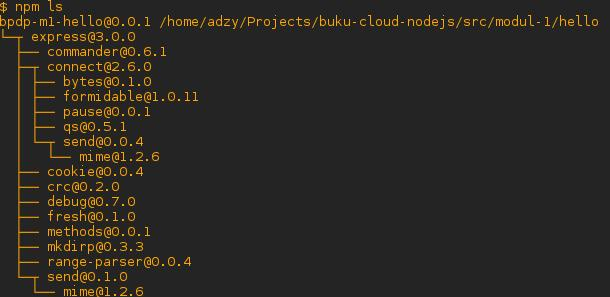
\includegraphics[scale=0.5]{images/npmls.jpg}
    \end{center}
    \caption{Hasil perintah npm ls}
    \label{fig:npmls}
  \end{figure}

\subsection{Menghapus Paket / \textit{Uninstall}}

Menghapus paket pustaka menggunakan npm pada dasarnya hampir sama dengan saat memasang paket, namun dengan perintah \textit{uninstall}. Berikut perintah lengkapnya.

\lstset{language=bash,caption=Perintah menghapus paket di npm}
\begin{lstlisting}
$ npm uninstall foo
\end{lstlisting}

Paket pustaka foo dalam lokal aplikasi akan dihapus, jika menggunakan hak administrasi sudo atau root maka akan menghapus dari installasi global.

\subsection{Berbagai Perintah Penting Pengelolaan Paket dengan npm}

